PageRank is an algorithm for assessing the significance of nodes within a network by assigning numerical scores based on link structures \cite{rank-page99}. It operates on the principle that pages with more high-quality inbound links are of greater importance and thus should have higher ranks. While originally devised to rank web pages in search results, this metric finds applications in various domains, such as urban planning \cite{urban-zhang18}, video object tracking \cite{gong2013pagerank}, traffic flow prediction \cite{traffic-kim15}, dynamic asset valuation \cite{sawilla2006abstracting}, protein target identification \cite{banky2013equal}\ignore{, brain region importance assessment \cite{zuo2012network}}, software system characterization \cite{chepelianskii2010towards}, and identification of crucial species for environmental health \cite{allesina2009googling}\ignore{, and quantifying the scientific impact of researchers \cite{rank-senanayake15}}.
% PageRank is a widely used centrality measure that "ranks" vertices in a graph by considering the connections and their importance. Efficiently updating PageRank for dynamic graphs is crucial in a number of applications, due to growing dataset sizes. However, traditional multicore CPUs have limited memory bandwidth, making them unfit for low computation-to-communication ratio algorithms like PageRank. GPUs, however, offer high-bandwidth memory and numerous lightweight cores with user-managed caches. This report introduces an efficient GPU implementation of Static PageRank and Dynamic Frontier with Pruning (DF-P) PageRank, which process only a subset of vertices likely to change ranks. On a server with a NVIDIA A100 GPU, our Static PageRank outperforms Hornet and Gunrock's PageRank implementations by $31\times$ and $5.9\times$ respectively, while being $24\times$ faster than our multicore Static PageRank. On top of the above, DF-P PageRank outperforms Static PageRank by $2.1\times$ on real-world dynamic graphs, and by $3.1\times$ on large static graphs with random batch updates.

With the rise of extensive interconnected data, interest in parallel PageRank computation algorithms has surged. These algorithms have been implemented across various platforms, including multicore CPUs \cite{rank-garg16, rank-beamer17, rank-lakhotia18, grutzmacher2020acceleration, huang2020accelerating, chen2021hipa}, GPUs \cite{duong2012parallel, rank-nvgraph, grutzmacher2018high, piccinotti2019solving, grutzmacher2020acceleration, kang2020computing, concessao2023meerkat}, FPGAs \cite{rank-guoqiang20}, SpMV ASICs \cite{rank-sadi18}, CPU-GPU hybrids \cite{rank-giri20}, CPU-FPGA hybrids \cite{usta2020accelerating, rank-li21, rank-hassan21, rank-mughrabi21}, and distributed systems \cite{rank-sarma13, kang2022analyzing, vandromme2022scaling}.

However, the dynamic nature of real-world graphs, characterized by frequent edge changes, presents challenges for recomputing PageRank. This is especially the case with small, rapid updates \cite{agarwal2012real, barros2021survey}. Existing strategies iterate from previous vertex ranks, reducing convergence iterations. To further minimize runtime, it's essential to recompute only likely changing vertex ranks. One prevalent approach involves identifying reachable vertices from updated graph regions and processing only these \cite{rank-desikan05, kim2015incremental, rank-giri20, sahu2022dynamic}. However, marking all reachable vertices as affected, even for minor changes, may lead to unnecessary computation, especially in dense graph regions. Our prior work \cite{sahu2024df} addressed these issues with parallel multicore algorithms. Here, we migrate these algorithms to GPUs, optimize for GPU-specific characteristics, and analyze the performance of the proposed dynamic PageRank algorithms.
% Unfortunately, multicore CPUs only offer a limited\ignore{parallelism and} memory bandwidth. This makes them unsuitable for graph algorithms, such as PageRank, which have a low computation-to-communication ratio. GPUs, on the other hand, boast extremely high bandwidth memory, connected in close proximity to thousands of lightweight cores with user-managed caches. Further, the GPU hardware is designed to be able to switch running threads at no cost in order to support memory access latency hiding. When graphs algorithms are suitably designed, they can significantly outperform a CPU-based implementation. This makes a GPU implementation of DF and DF-P PageRank attractive. In this section, we describe the design of DF and DF-P PageRank for GPU.




\subsection{Our Contributions}

This report presents our improved Dynamic Frontier (DF) and Dynamic Frontier with Pruning (DF-P) approaches\footnote{\url{https://github.com/puzzlef/pagerank-cuda-dynamic}} for updating PageRank on dynamic graphs. These approaches efficiently identify vertices likely to change ranks upon batch updates, with minimal overhead. On a server with a 64-core AMD EPYC-7742 processor, our approaches outperform Static and Dynamic Traversal PageRank by $5.2\times$/$15.2\times$ and $1.3\times$/$3.5\times$ respectively on real-world dynamic graphs, and by $7.2\times$/$9.6\times$ and $4.0\times$/$5.6\times$ on large static graphs with random batch updates. Our observations indicate that the speedup offered by DF and DF-P PageRank mainly stems from the incremental marking of affected vertices. Additionally, our approaches show performance gains of $1.8\times$/$1.7\times$ for every doubling of threads.

\begin{table}[hbtp]
  \centering
  \caption{Speedup of our GPU implementation of Static PageRank compared to other state-of-the-art implementations. Direct comparisons are based on running the given implementation on our server, while indirect comparisons (denoted with a $*$) involve comparing results obtained by the given implementation relative to a common reference (Hornet/Gunrock).}
  \label{tab:compare-large}
  \begin{tabular}{|c|c||c|}
    \toprule
    \textbf{PageRank implementation} &
    \textbf{Published} &
    \textbf{Our Speedup} \\
    \midrule
    Hornet \cite{busato2018hornet} & 2018 & $31\times$ \\ \hline
    Gunrock \cite{wang2016gunrock} & 2016 & $5.9\times$ \\ \hline
    Galois with Gluon \cite{dathathri2018gluon} & 2018 & $448\times^*$ \\ \hline
    Tigr \cite{nodehi2018tigr} & 2018 & $40\times^*$ \\ \hline
    Grus \cite{wang2021grus} & 2021 & $7.2\times^*$ \\ \hline
    Atos \cite{chen2022atos} & 2022 & $7.6\times^*$ \\ \hline
    Multi-GPU Atos ($1$ GPU) \cite{chen2022scalable} & 2022 & $7.8\times^*$ \\ \hline
    Multi-GPU Atos ($4$ GPUs) \cite{chen2022scalable} & 2022 & $4.8\times^*$ \\ \hline
    GraphBLAST \cite{yang2022graphblast} & 2022 & $11\times^*$ \\ \hline
    Meerkat \cite{concessao2023meerkat} & 2023 & $18\times^*$ \\ \hline
  \bottomrule
  \end{tabular}
\end{table}

\begin{table}[hbtp]
  \centering
  \caption{Speedup of our GPU implementation of Dynamic Frontier with Pruning (DF-P) PageRank compared to other approaches of updating PageRank scores (on GPU), on real-world dynamic graphs (Table \ref{tab:dataset}), and on large static graphs with random batch updates (Table \ref{tab:dataset-large}), respectively.}
  \label{tab:compare}
  \begin{tabular}{|l||c|}
    \toprule
    \textbf{PageRank approach} &
    \textbf{Speedup of DF-P} \\
    \midrule
    Static \cite{rank-page99} & $2.1\times$, $3.1\times$ \\ \hline
    Naive-dynamic (ND) \cite{rank-page99, rank-zhang17} & $1.5\times$, $1.7\times$ \\ \hline
    Dynamic Traversal (DT) \cite{rank-desikan05, kim2015incremental, rank-giri20, sahu2022dynamic} & $1.8\times$, $13.1\times$ \\ \hline
    Dynamic Frontier (DF) \cite{sahu2024df} & $2.1\times$ $1.3\times$ \\ \hline
  \bottomrule
  \end{tabular}
\end{table}





%% - Use --- for a dash.
%% - Use ``camera-ready'' for quotes.
%% - Use {\itshape very} or \textit{very} for italicized text.
%% - Use \verb|acmart| or {\verb|acmart|} for mono-spaced text.
%% - Use \url{https://capitalizemytitle.com/} for URLs.
%% - Use {\bfseries Do not modify this document.} for important boldface details.
%% - Use \ref{fig:name} for referencing.

%% For a block of pre-formatted text: 
% \begin{verbatim}
%   \renewcommand{\shortauthors}{McCartney, et al.}
% \end{verbatim}

%% For a list of items:
% \begin{itemize}
% \item the ``ACM Reference Format'' text on the first page.
% \item the ``rights management'' text on the first page.
% \item the conference information in the page header(s).
% \end{itemize}

%% For a table:
% \begin{table}
%   \caption{Frequency of Special Characters}
%   \label{tab:freq}
%   \begin{tabular}{ccl}
%     \toprule
%     Non-English or Math&Frequency&Comments\\
%     \midrule
%     \O & 1 in 1,000& For Swedish names\\
%     $\pi$ & 1 in 5& Common in math\\
%     \$ & 4 in 5 & Used in business\\
%     $\Psi^2_1$ & 1 in 40,000& Unexplained usage\\
%   \bottomrule
% \end{tabular}
% \end{table}

%% For a full-width table:
% \begin{table*}
%   \caption{Some Typical Commands}
%   \label{tab:commands}
%   \begin{tabular}{ccl}
%     \toprule
%     Command &A Number & Comments\\
%     \midrule
%     \texttt{{\char'134}author} & 100& Author \\
%     \texttt{{\char'134}table}& 300 & For tables\\
%     \texttt{{\char'134}table*}& 400& For wider tables\\
%     \bottomrule
%   \end{tabular}
% \end{table*}


%% For inline math:
% \begin{math}
%   \lim_{n\rightarrow \infty}x=0
% \end{math},

%% For a numbered equation:
% \begin{equation}
%   \lim_{n\rightarrow \infty}x=0
% \end{equation}

%% For an unnumbered equation:
% \begin{displaymath}
%   \sum_{i=0}^{\infty} x + 1
% \end{displaymath}

%% For a figure:
% \begin{figure}[h]
%   \centering
%   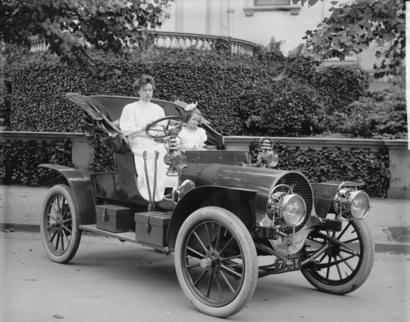
\includegraphics[width=\linewidth]{inc/sample-franklin}
%   \caption{1907 Franklin Model D roadster. Photograph by Harris \&
%     Ewing, Inc. [Public domain], via Wikimedia
%     Commons. (\url{https://goo.gl/VLCRBB}).}
%   \Description{A woman and a girl in white dresses sit in an open car.}
% \end{figure}

%% For a teaser figure.
% \begin{teaserfigure}
%   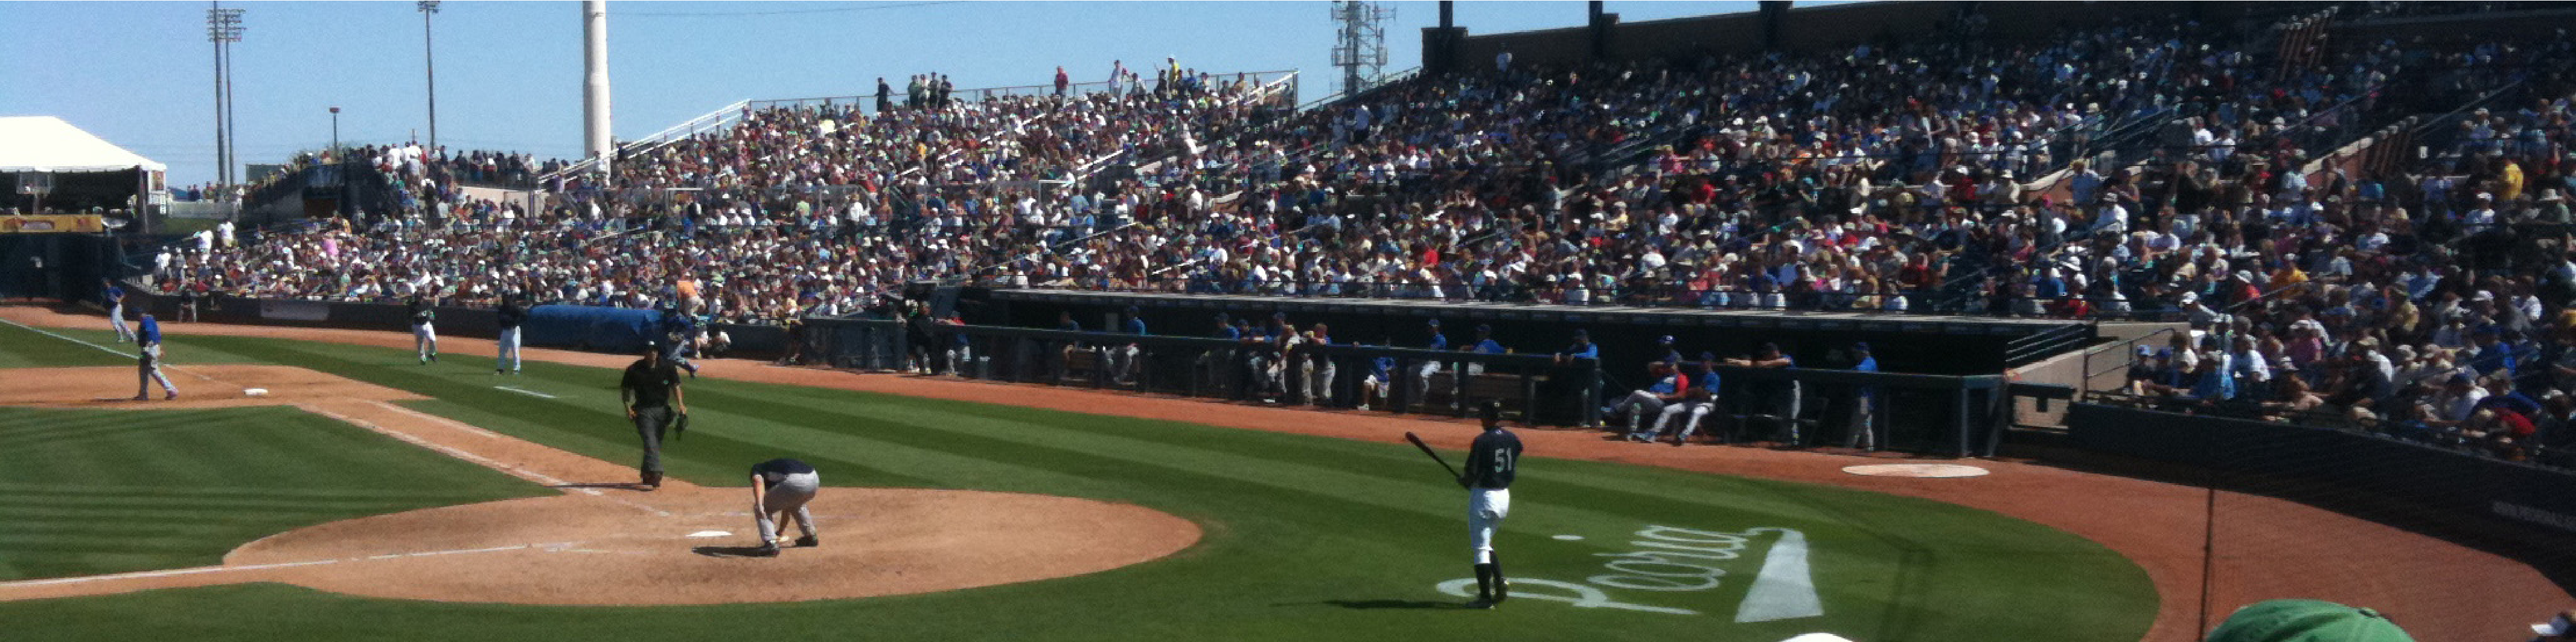
\includegraphics[width=\textwidth]{sampleteaser}
%   \caption{figure caption}
%   \Description{figure description}
% \end{teaserfigure}
